%RATIOS \& RATES INTRODUCTION - WORKSHEET 0 (IN-CLASS INSTRUCTION)
\documentclass[12pt, letterpaper, fleqn]{article}

% ----------------------------------------------------------
% PACKAGES
% ----------------------------------------------------------
\usepackage{graphicx}
\usepackage{xcolor}
\usepackage[most]{tcolorbox}
\usepackage{amsmath, amssymb}
\usepackage{fancyhdr}
\usepackage[utf8]{inputenc}
\usepackage[T1]{fontenc}
\usepackage{enumitem}
\usepackage{geometry}
\usepackage{tikz}
\usepackage{needspace}
\usepackage{multicol}

\usetikzlibrary{arrows.meta, calc}

% ----------------------------------------------------------
% PAGE SETUP
% ----------------------------------------------------------
\usepackage{times}
\geometry{letterpaper, top=1.25in, bottom=1.25in, marginpar=0.5in}

% ----------------------------------------------------------
% HEADER / FOOTER
% ----------------------------------------------------------
\newcommand{\logowidth}{3cm}
\setlength{\headheight}{20pt}
\setlength{\footskip}{40pt}

\pagestyle{fancy}
\fancyhf{}
\fancyhead[C]{\small\bfseries Ratios \& Rates Introduction}
\fancyfoot[L]{\raisebox{2pt}{
\includegraphics[width=\logowidth]{kss.png}}}
\fancyfoot[C]{\thepage}
\fancyfoot[R]{6.1.0}

\renewcommand{\footrulewidth}{0.2pt}

% ----------------------------------------------------------
% THEME COLOR
% ----------------------------------------------------------
\definecolor{customteal}{HTML}{2fbdb9}

% ----------------------------------------------------------
% HELPER MACROS
% ----------------------------------------------------------
\newcommand{\blank}{\underline{\hspace{2.2cm}}}
\newcommand{\blanklong}{\underline{\hspace{6.5cm}}}
\newcommand{\blankshorter}{\underline{\hspace{1.5cm}}}

% ----------------------------------------------------------
% DOCUMENT
% ----------------------------------------------------------
\begin{document}


\textbf{Name:} \underline{\hspace{5cm}}
\hfill
\textbf{Date:} \underline{\hspace{3cm}}\\

% ==========================================================
% SECTION 1: WHAT IS A RATIO?
% ==========================================================
\begin{tcolorbox}[colback=customteal!20]
    \large\textcolor{black}{\textbf{What is a Ratio? (Foundation)}}
\end{tcolorbox}

\vspace{3mm}

\noindent
A \textbf{ratio} is a comparison between two quantities. Ratios tell us how much of one thing there is compared to another.

\begin{itemize}
    \item A ratio of 2 boys to 3 girls means: for every 2 boys, there are 3 girls
    \item A ratio of 5 apples to 2 oranges means: for every 5 apples, there are 2 oranges
    \item We can write ratios three ways: ``2 to 3'', ``2:3'', or $\dfrac{2}{3}$
\end{itemize}

\medskip

\noindent
\textbf{Two Types of Ratios:}
\begin{enumerate}
    \item \textbf{Part-to-Part Ratio:} Compares one part to another part
    \begin{itemize}
        \item Example: ``3 red buttons to 5 blue buttons'' (red compared to blue)
    \end{itemize}
    
    \item \textbf{Part-to-Whole Ratio:} Compares a part to the whole
    \begin{itemize}
        \item Example: ``3 red buttons to 8 total buttons'' (red compared to all)
    \end{itemize}
\end{enumerate}

\vspace{4mm}

% ==========================================================
% VISUAL REPRESENTATION
% ==========================================================
\begin{tcolorbox}[colback=white, colframe=black!25, boxrule=0.6pt, arc=4mm, left=6mm, right=6mm, top=5mm, bottom=5mm]

\textbf{Example: Buttons in a Jar}

\medskip

\begin{center}
\begin{tikzpicture}[scale=0.8]
% Draw buttons
\foreach \i in {1,2,3} {
    \draw[fill=red!70] (\i*0.8, 1) circle(0.25);
}
\foreach \i in {1,2,3,4,5} {
    \draw[fill=blue!70] (\i*0.8, 0) circle(0.25);
}
\node at (0, -0.8) {3 red};
\node at (2, -0.8) {5 blue};
\node at (4, -0.8) {8 total};
\end{tikzpicture}
\end{center}

\medskip

\noindent
\textbf{Part-to-Part Ratio:} Red to Blue = $3:5$ or ``3 to 5''
\\

\noindent
\textbf{Part-to-Whole Ratio:} Red to total = $3:8$ or ``3 to 8''


\end{tcolorbox}

\vspace{4mm}

% ==========================================================
% PRACTICE 1: IDENTIFYING RATIOS
% ==========================================================
\newpage
\begin{tcolorbox}[colback=customteal!20]
\large\textcolor{black}{\textbf{Practice: Write Ratios}}
\end{tcolorbox}

\noindent
For each situation, write the ratio two ways.

\vspace{3mm}

\begin{enumerate}[itemsep=1.5cm, leftmargin=0.6cm]

\item In a class, there are 12 boys and 15 girls.
\vspace{1cm}
\begin{itemize}
    \item Boys to girls: \blank : \blank
    \vspace{1cm}
    \item Girls to all students: \blank : \blank
\end{itemize}

\item A fruit bowl has 4 apples, 6 oranges, and 5 bananas.
\vspace{1cm}
\begin{itemize}
    \item Apples to oranges: \blank : \blank
    \vspace{1cm}
    \item Apples to all fruit: \blank : \blank
\end{itemize}

\item A store has 2 chefs and 6 waiters.
\vspace{1cm}
\begin{itemize}
    \item Waiters to chefs: \blank : \blank
    \vspace{1cm}
    \item Chefs to all employees: \blank : \blank
\end{itemize}

\end{enumerate}

\newpage

% ==========================================================
% SECTION 2: USING RATIO LANGUAGE
% ==========================================================
\begin{tcolorbox}[colback=customteal!20]
\large\textcolor{black}{\textbf{Using Ratio Language}}
\end{tcolorbox}

\noindent
When we say ``the ratio of A to B is 2:3'', we mean: \textbf{For every 2 units of A, there are 3 units of B.}

\vspace{3mm}

\begin{tcolorbox}[colback=white, colframe=black!25, boxrule=0.6pt, arc=4mm, left=6mm, right=6mm, top=5mm, bottom=5mm]

\textbf{Worked Example 1: Recipe}

\medskip

\textbf{Problem:} A juice recipe uses a ratio of 2 cups of water to 1 cup of juice concentrate.

\noindent
If we want to make double the recipe, how much of each ingredient do we need?

\medskip

\noindent
\textbf{Solution:}

\medskip

\noindent
Double means multiply everything by 2:
\begin{itemize}
    \item Water: $2 \times 2 = 4$ cups
    \item Juice concentrate: $1 \times 2 = 2$ cups
\end{itemize}

\medskip

\noindent
The ratio stays the same: $4:2$ is the same as $2:1$ (double the amount).

\end{tcolorbox}

\vspace{4mm}

% ==========================================================
% THINKING PROBLEM 1
% ==========================================================
\begin{tcolorbox}[colback=white!15, colframe=black, boxrule=1.5pt, arc=4mm, left=6mm, right=6mm, top=5mm, bottom=5mm]

\textbf{Deeper Thinking Problem 1: Recipe Scaling}

\medskip

\noindent
A cookie recipe calls for a ratio of 3 cups flour to 2 cups sugar.

\noindent
\textbf{a)} What is the ratio of sugar to flour?

\vspace{3cm}

\noindent
\textbf{b)} If you use 9 cups of flour, how much sugar do you need?

\vspace{3cm}

\end{tcolorbox}

\newpage

% ==========================================================
% SECTION 3: REPRESENTING RATIOS
% ==========================================================
\begin{tcolorbox}[colback=customteal!20]
\large\textcolor{black}{\textbf{Different Ways to Show a Ratio}}
\end{tcolorbox}

\noindent
The same ratio can be shown with words, a colon, or a fraction. They all mean the same thing.

\vspace{3mm}

\begin{tcolorbox}[colback=white, colframe=black!50, boxrule=0.6pt, arc=4mm, left=6mm, right=6mm, top=5mm, bottom=5mm]

\textbf{Example: Three Ways to Write a Ratio}

\medskip

\begin{enumerate}
    \item \textbf{Words:} ``3 to 5''
    \item \textbf{Colon notation:} $3:5$
    \item \textbf{Fraction:} $\dfrac{3}{5}$
\end{enumerate}

\medskip

\noindent
All three mean the same thing: for every 3 of one thing, there are 5 of another.

\end{tcolorbox}

\vspace{4mm}

% ==========================================================
% THINKING PROBLEM 2
% ==========================================================
\begin{tcolorbox}[colback=white!15, colframe=black, boxrule=1.5pt, arc=4mm, left=6mm, right=6mm, top=5mm, bottom=5mm]

\textbf{Deeper Thinking Problem 2: Sports Teams}

\medskip

\noindent
At a basketball tournament, the ratio of boys' teams to girls' teams is 4:3.

\noindent
\textbf{a)} If there are 16 boys' teams, how many girls' teams are there?

\vspace{4cm}

\noindent
\textbf{b)} What is the total number of teams?

\vspace{4cm}

\end{tcolorbox}

\newpage

% ==========================================================
% SECTION: EQUIVALENT RATIOS
% ==========================================================
\begin{tcolorbox}[colback=customteal!20]
\large\textcolor{black}{\textbf{Equivalent Ratios}}
\end{tcolorbox}

\noindent
Ratios are equivalent when both numbers are multiplied or divided by the same amount.

\vspace{3mm}

\begin{tcolorbox}[colback=white, colframe=black!25, boxrule=0.6pt, arc=4mm, left=6mm, right=6mm, top=5mm, bottom=5mm]

\textbf{Worked Example}

\medskip

Is $2:3$ equivalent to $4:6$?

\[
2 \times 2 = 4
\]

\[
3 \times 2 = 6
\]

Since both parts were multiplied by 2, the ratios are equivalent.

\[
2:3 = 4:6
\]


\end{tcolorbox}

\vspace{4mm}

\begin{tcolorbox}[colback=white!15, colframe=black, boxrule=1.5pt, arc=4mm, left=6mm, right=6mm, top=5mm, bottom=5mm]

\textbf{Practice: Equivalent or Not?}

\medskip

\noindent
\textbf{a)} Is $3:5$ equivalent to $6:10$? Explain.

\vspace{3cm}

\noindent
\textbf{b)} Is $4:7$ equivalent to $8:15$? Explain.

\vspace{3cm}

\end{tcolorbox}

\newpage

% ==========================================================
% THINKING PROBLEM 3
% ==========================================================
\begin{tcolorbox}[colback=white!15, colframe=black, boxrule=1.5pt, arc=4mm, left=6mm, right=6mm, top=5mm, bottom=5mm]

\textbf{Deeper Thinking Problem 3: School Colors}

\medskip

\noindent
A school is ordering decorations. The ratio of red decorations to blue decorations is 5:2.
\noindent
\vspace{1cm}

\textbf{a)} If they order 50 red decorations, how many blue decorations do they need?

\vspace{2cm}
\vspace{3cm}

\noindent
\textbf{b)} How many decorations total?
\vspace{2cm}
\vspace{3cm}

\noindent
\textbf{c)} What fraction of all decorations are red? (Hint: use part-to-whole)
\vspace{2cm}
\vspace{3cm}

\end{tcolorbox}


\end{document}
\end{document}
